\documentclass{article}
\usepackage{lmodern} % Latin Modern Font
\usepackage[T1]{fontenc}
\usepackage{amsfonts} % \mathbb
\usepackage[margin=0.5in]{geometry}
\usepackage[utf8]{inputenc}
\usepackage{graphicx}
\usepackage[backend=biber, style=apa]{biblatex}
\usepackage{amsmath}
\usepackage{amssymb} % blackbox symbol
\usepackage{hyperref}
\usepackage{hypcap}
\DeclareMathOperator{\sign}{sign}
\bibliography{bibli}
\hypersetup{
  colorlinks=true, 
  allcolors=black,
  pdfauthor={Carlos Tarjano},
  pdftitle={Robust Digital Envelope Estimation Via Geometric Properties of an Arbitrary Real Signal}
}
\title{Robust Digital Envelope Estimation Via Geometric Properties of an Arbitrary Real Signal}
\author{Carlos Tarjano \and Valdecy Pereira}

\begin{document}

\maketitle

\begin{abstract} % 250 words
% background  
Despite being an elusive concept, the temporal amplitude envelope of a signal is essential for its complete characterization, being the primary information carrying medium in spoken voice and telecommunications, for example.
intuitively, the temporal envelope can be understood as a smooth function, that modulates the signal, being responsible for its outer shape.
% motivation
Envelope detection techniques have applications in areas like health, sound classification and synthesis, seismology and speech recognition. Despite of that, a general approach to envelope detection of signals with rich spectral content seems to be lacking, and most methods involve manual intervention, like filter design or smoothing, based on prior knowledge about the wave under investigation.
% objective
In this paper we propose a framework that uses intrinsic characteristics of a signal to estimate its envelope, completely eliminating the necessity of parameter tuning.
% methods
The approach here described draws inspiration from general, computational and differential geometry to isolate the frontiers and thus estimate the temporal envelope of an arbitrary signal; to that end The concepts of alpha-shapes, concave hulls, and discrete curvature are explored. We also define a pulse in the context of a arbitrary digital signal as a means to reduce dimensionality and the complexity of the proposed algorithm.
% results
We find the algorithm accurate in the identification of the frontiers of a wide range of digital sound signal with very diverse characteristics, while providing the dominant frequency of the wave as a by-product. The algorithm also compares favourably with a common detection technique based on the Hilbert Transform.
While the results are satisfactory per se, we define several geometric entities in this work, including a new measure of discrete curvature; hoping to consolidate theory in the area, while providing a solid basis for the development of new techniques, specially in sound synthesis and classification.
\end{abstract}

{\bf Keywords:} DSP, alpha-shapes, envelope detection

\section{Introduction} % 500 words
% Opener sentence
Despite being ubiquitous in both analog and digital signal processing \parencite{2011CaetanoImproved}, the literature about envelope detection is very fragmented \parencite{2017LyonsDigital}. Besides, most envelope detection techniques are designed to account for very specific settings, like pure sinusoids with moderate noise contents, in line with the most common usages of those algorithms with artificial signals in the context of analog telecommunications; that limitation arises in part by the lack of a mathematical definition for a temporal envelope \parencite{2013Mengempirical}.

% Literature review | Brief Context of Prior Research
In many natural signals, however, the temporal amplitude envelope of a signal plays a prominent role in the characteristics exhibited: According to \textcite{2017QiRelative}, for example, the envelope is at least as important as the fine structure of the soundwave in the context of the intelligibility of mandarin tones. That is also the case for English \parencite{1995ShannonSpeech}, where even envelopes modulating mostly noise were still capable of conveying meaning. 

The envelope helps to convey emotion and identity to the human voice \parencite{2018ZhuContributions}, and envelope preserving characteristics of concert halls are associated with their pleasantness \parencite{2011LokkiEngaging}.

% Cite current algorithms
When dealing with broadband signals, approaches tailored to specific applications are prevalent, such as the one presented by \textcite{2014YangFast} for the distributed monitoring of fibre optic or the one formulated by \textcite{2018AssefModeling} in the context of medical ultrasound imaging.

If one adresses the different units in the horizontal and vertical axes, one can transform the DSP problem of envelope detection in the geometric problem of defining the shape of a set of points in $ \mathbb{R}^2 $. For that purpose \textcite{1983Edelsbrunnershape} introduced the concept of alpha-shapes, a mathematically well defined extension to the convex hull of a finite set of points, related to the Delaunay triangulation and Voronoi diagrams of those points.

This approach is used in areas such as the detection of features in images \parencite{2016VarytimidisAlpha}, reconstruction of surfaces from a cloud of points \parencite{2015WuAutomated} and Spectroscopy \parencite{2019XuModeling}, with the last work, that involves the estimation and removal of the Blaze function (a kind of envelope) of a echelle spectrograph, being particularly align with what is intended here.

Interesting steps in the direction of translating geometric algorithms to the context of envelope detection were made by \textcite{2015YangSkeleton} with an approach based on the construction of a skeleton underlying the wave, and with the direct translation of computer vision methods to the task \parencite{2015YangRepresenting}.

% Restate Your Question as Something Not Known or Fully Understood by Prior Research
Thus, in this paper we formulate a general approach to envelope detection, exploiting the intrinsic characteristics of a generic, spectrally complex, wave in order to avoid the need to manual intervention or parameter tuning.

% State the Significance of Your Question
While the robustness of the proposed approach allows it to be used as a plug in replacement for many methods encountered in the literature, we feel that it would be particularly useful for sound synthesis; the envelope is shown to add complexity to the spectral representation of a wave \parencite{2019TarjanoNeuro}, and a accurate description of the envelope would be useful for a cleaner spectral analysis. Moreover, the algorithm naturally divides a signal in pseudo-cycles, that could serve pragmatic building blocks for the reconstruction of the fine structure of the wave.

% State Your Claim | Objective | Hypothesis
In the context of sound synthesis, for example, one would be able to apply specific methods for the recreation of the envelope, more in line with its smooth, slow varying and non periodic nature and a different approach to the periodic and relatively fast changes of the temporal fine structure.

% brief outlook on the structure of the paper
After explaining and defining the various entities used later, of which the concept of frontiers is arguably the most important, in the methodology section, we dedicate a section to present a new discrete curvature estimation approach.
We proceed to illustrate the results of the application of the algorithm in a set of 6 diverse sound waves, ranging from voice to unpitched instruments.

We then discuss the future implications of the work, emphasizing the focus on the construction of new interpretations of the relation between time domain and frequency domain sound descriptions, and our vision of the impact of this methodology in the field of sound synthesis.
A range of potential future developments is also presented.


\section{Methodology} % 1000 words

% Essential background information
In this work it is assumed, without loss of generality, that one is interested in retrieving the mathematically ill defined \parencite{2013Mengempirical} temporal envelope of a arbitrary physical sound wave, of which only a recording is available. 

Naturally, due to the necessary truncations both in time and in amplitude, as well as measure errors introduced by the instruments used to record the signal, it is not possible to characterise exactly the original, continuous wave, from its digital counterpart.

The best representation one can hope to get of the original wave is, then, the original recording. It is sensible, thus, to characterise the envelope of that wave in terms of a subset of the exact samples that comprise the digital representation.

To that end, this work will emphasize the concept of frontier, as the points of the digital wave that mark the wave's upper and lower boundaries; from those points an envelope, conforming to the vague definitions of uniqueness and smoothness, can be trivially constructed.

We start by defining a pulse as a series of consecutive samples in a discrete wave with the same sign. More formally, let $ W[i] \in \mathbb{R} \ \forall \ i \in \mathbb{N}_0, \ i < n \in \mathbb{N}_0 $ be a real, discrete and finite signal indexed, without loss of generality, over a adjacent subset of the natural numbers starting at zero. This definition relates closely to the concept of an array or vector in most programming languages, and is used in the interest of simplicity.

A pulse $ P[j], j \in \mathbb{N}_0, j < q $ in $ W $ can then be defined as a sequence of samples indexed by $ i $ such that $ \sign(W[a-1]) \ne \sign(W[a]) = \sign(W[a+1]) = \dots = \sign(W[b-1]) = \sign(W[b]) \ne \sign(W[b+1]) \forall i, a \le i \le b | a,b \in \mathbb{N}_0 $.

In other words, each pulse is a unique subset of $ W $ with its members being the maximum sequence of samples in $ W $ with the same signal and $ P[0] \cup P[1] \cup \cdots \cup P[q-1] = W $. It is convenient to attribute to each pulse a pair of coordinates: those will be the coordinates of the sample with the maximum absolute amplitude in each pulse, being denoted by $ P[j]_x $ and $ P[j]_y $; additionally, the length of a pulse will be denoted by $ P[j]_l $.

Naturally, each pulse can be classified as positive or negative, based on the sign of its samples, which must be the same.
For a continuous function, then, a pulse would correspond to the pieces between its roots, and would be equal to half the cycle of a sinusoid. Thus, in our analogy, two consecutive pulses, naturally with opposing signs, have the potential do delimitate a pseudo-cycle, as illustrated in figure \ref{fig:Pulses}. For that to be true, however, the pulses need to make part of the frontiers of the signal, as will be defined later.

  \begin{figure}[ht!]
    \centering
      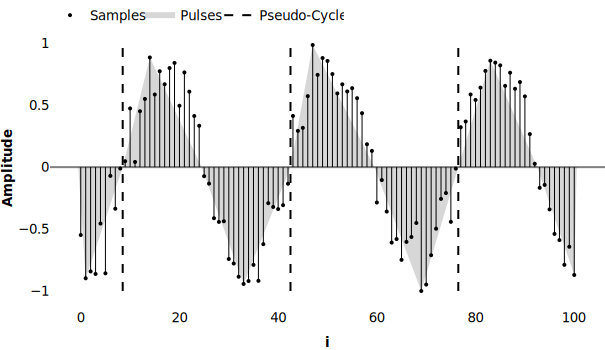
\includegraphics[width=0.8\linewidth]{01Pulses.pdf}
    \caption{The grey areas encompass the simplified convex hulls of the pulses. The dashed lines mark the frontier between pseudo-cycles.}
    \label{fig:Pulses}
  \end{figure}

The most mathematically sound definition of an envelope involves its representation as an analytic signal, introduced by Gabor in 1946 \parencite{2007HahnHistory}. In his work, \textcite{1946GaborTheory} applies the then relatively new mathematical machinery of the quantum mechanics to unify time and frequency representations of a wave, showing how the Hilbert transform could be applied to a real signal in order to obtain a complex signal that would become known as the analytic signal.

This analytic signal is of the form $ a(t) = s(t) + \mathbb{H}(s(t)) \ \text{i} $ \parencite{2016HePraat} where $ s(t) $ is the original real signal, that becomes the real part of the analytic signal. $ \mathbb{H}(s(t)) $, the Hilbert transform of the original signal becomes, then, the imaginary part of the analytic signal; the envelope of a signal thus represented can be straightforwardly obtained by the computation of its complex modulus.

\begin{figure}[ht!]
  \centering
    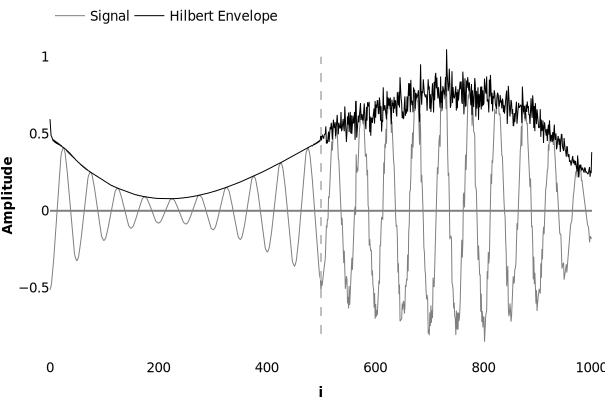
\includegraphics[width=0.8\linewidth]{02AnalyticSignal.pdf}
  \caption{Envelope of a pure sinusoid modulated by a polynomial of degree 3, as obtained by the Hilbert Transform. In the first half the sinusoid is free of noise, while in the second half white gaussian noise with a standard deviation of $ 1/10 $ of the maximum amplitude of the wave was added to the base signal.}
  \label{fig:AnalyticSignal}
\end{figure}

Figure \ref{fig:AnalyticSignal} shows the envelope obtained via the Hilbert transform, for a pure sinusoid of local frequency 20, modulated by a polynomial of the third degree, in the presence and absence of gaussian white noise with standard deviation of $ 1/10 $ of the wave's maximum amplitude. It is readily noticeable that, as soon as noise is introduced in the original signal, it is reflected in the envelope, breaking our assumption of smoothness. Other than that, this definition yields a unique, positive envelope.

In practice, however, is not uncommon for a discrete wave, specially in the case of sound, to present somewhat different positive and negative contours; as our method will forcibly have to be applied separately to both sides, superior and inferior, of the discrete wave, it is only natural to introduce such separation as soon as possible. 

To do so we will define the positive (upper) frontier and negative (lower) frontier as the set of points $ (i, |W[i]|) $ that are, necessarily but not sufficiently, the points of maximum absolute amplitude of their respective pulses. The set of all these points such that $ W[i] > 0 $ will be called the positive, piecewise linear frontier and will be denoted by $ F^+ $; similarly, $ F^- $ will denote the negative frontier of $ W $, defined by the subset of points $ (i, W[i]) $ where $ W[i] < 0 $, as is shown in figure \ref{fig:Frontiers}. To identify such points, we need to address the different units in which the amplitude and horizontal distance of our wave are expressed.

\begin{figure}[ht!]
  \centering
    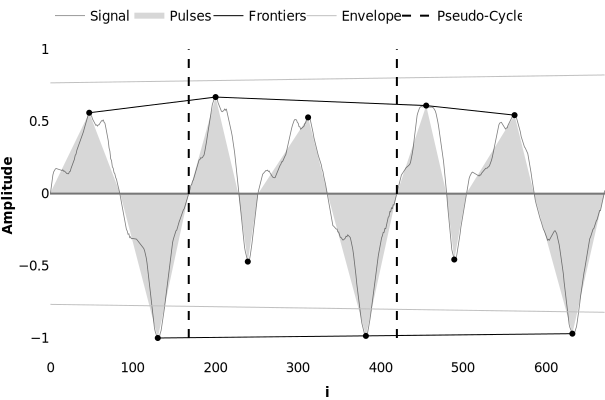
\includegraphics[width=0.8\linewidth]{03Frontiers.pdf}
  \caption{Positive and negative frontiers, envelope and pseudo-cycles for a fragment of piano sound. While we have only one (positive) envelope, here mirrored in the inferior space, we have two frontiers, the superior and inferior.}
  \label{fig:Frontiers}
\end{figure}

To make abscissa and ordinate units consistent for the computation of the frontier, and proceed with a geometric treatment of the subject, we consider the set of positive and negative pulses separately. For each set, we multiply all pulses lengths by the average length of the pulses in the set, after having divided by the average of the pulses' amplitudes, putting both axes in the same unit $i$, related to time by the equation $i = t \ \mathit{fps}$.

Formally, supposing we have $ m $ pulses with the same sign, we scale each pulse's vertical coordinate by $s$, where:

\begin{equation} \label{eq:scale}
  s = \frac{\sum_{i=1}^{m} P[i]_l}{\sum_{i=1}^{m} P[i]_y}
\end{equation}

Because we are interested in approximating a function that is smooth over the whole domain of the wave, we can assume that, in the scale of a pulse, this function will be very close to a horizontal straight line and, thus, won't touch any point inside the convex hull defined by the pulse. 

By the same token, as the change in amplitude from one pulse to the next pulse with the same sign is motivated by changes in this same envelope, one can reasonably suppose that $ \max(P[j]) \approx \max(P[j+2]) $. That justifies the approximation of the convex hull of a pulse by the triangle defined by the points where the pulse crosses the horizontal the point of maximum amplitude; this will allow a considerable dimension reduction as this triangular pulse can become the atomic unit for the rest of the method. 

This definition also makes clear that only one point of an arbitrary pulse can be in the frontier, namely, its point of maximum amplitude; those definitions will allow us to derive the frontiers of a wave using an alpha-shapes inspired algorithm without the need to compute the Delaunay triangulation first.

Translating the intuitive explanation of alpha-shapes in \textcite{1994EdelsbrunnerThree} to our context, we can say that the points in the frontier are those touched by a circle outside the signal that is not allowed to contain any point of the signal; The pulses that contain said points can be seen as frontier pulses.
Intuitively, one can picture a circle being rolled above (or below, in the case of the negative frontier) the signal, and marking the points it touches as frontier points.

We can therefore revisit the concept of a pseudo-cycle, only hinted at before, defining it as the samples of the original wave that belong to two successive pulses that belong to their respective frontiers, including eventual pulses between them, as can be seen in figure \ref{fig:Frontiers}.

It is now necessary to infer the appropriate radius of such a circle and, to that end, a measure of the curvature of a discrete function is needed. Discrete curvature estimation is an important task in image processing \parencite{2010FleischmannNovel} for which no default definition exists; The two possible approaches are the derivation of direct methods that use characteristics of the discrete wave to calculate its curvature at each point, or the calculation of the curvature of a curve fitted to the discrete wave \parencite{2001CoeurjollyDiscrete}.

To fit a polynomial to the a generic wave two approaches are readily available: the least mean squares approach, that seeks to minimize the dependant variable errors and the total least squares problem, that treats both variables symmetrically \parencite{1980GolubAnalysis}.

The geometric, symmetrical nature of the problem excludes the more computationally economic least mean squares approach however, leaving us with the total least squares, for which no general closed form solutions are available \parencite{2007MarkovskyOverview}; this leads us to turn our attention to direct approaches of curvature estimation.

\subsection{Discrete Curvature Estimation - The Equivalent Circle Approach}

As previously stated, no default discrete curvature definition exists; \textcite{2014CarrollSurvey}, for example, derives 3 such different definitions based on the approximation of a circle by an inscribed, centred e circumscribed polygon. In the context of 3d meshes, \textcite{2016VasaMultivariate} evaluate a range of estimators from a multivariate point o view.

For our needs, however, it is more convenient to define our own discrete curvature estimator; the approach here presented differs from most others found in the literature in that the curvature is defined over the edges linking the points that form the discrete wave, instead of the vertices.

To that end we are going to apply the definition of smooth curvature as the rate of change of the unit tangent to a curve, noting that this is equivalent to that of the osculating circle \parencite{2016VasaMesh}.
The idea is to find the equivalent circle whose tangent presents the same change in direction, in the same horizontal distance, as the edge of interest. This approach presents the convenience of estimating the radius directly.

\begin{figure}[ht!]
  \centering
    \includegraphics[width=0.3\linewidth]{04DiscreteCurvature.pdf}
  \caption{Change of direction from horizontal, in $ \hat{u}_0 $, until an angle of $ \theta $, in $ \hat{u}_1 $, that is equivalent to the angle between the average direction and the direction of the vector $ \vec{v}_l $ whose radius of curvature is being calculated, shown in the picture in grey.}
  \label{fig:DiscreteCurvature}
\end{figure}

Formally, for each frontier, positive or negative, we define $ m-1 $ vectors, $ m $ being the number of positive or negative pulses respectively, as the coordinates of the posterior pulse with the relevant signal minus the preceding pulse: $\vec{v}_l^\pm = (P[l+1]_x^\pm - P[l]_x^\pm, P[l+1]_y^\pm - P[l]_y^\pm), \forall 0 \ \le l < m - 1 $, recalling that the $x$ coordinate of a pulse was defined as the $x$ coordinate of its sample with maximum amplitude, while the $y$ coordinate of a pulse is this amplitude itself.

Since an edge defines only one direction, there remains the need for a direction of reference. As we are interested in the relative curvature, it is natural to use the average direction of all positive or negative vectors, $ \vec{\overline{v}}^\pm = \frac{1}{m-1} \sum_{l=0}^{m-1} \vec{v}_l^\pm $, so as to measure the relative change of direction of each edge. This procedure, as well as the circles generated by it, are illustrated in figure \ref{fig:Curvatures}. 

The angle $ \theta $ between the average direction and each of the vectors can be obtained via the relation between the slopes of the respective lines, as in the expression $ \theta = \arctan( (m - \overline{m}) / (1 + m \overline{m}) ) $. The radii of the equivalent circles are thus given by $ r_l = x_l / \sin (\theta_l) $ with the curvature given by $\kappa_l =1/r_l=\sin (\theta_l) / x_l$. After some algebra, one can write:

\begin{equation} \label{eq:radius}
  r_l = \left\lvert \frac{x_l \sqrt{\overline{m}^2 + 1} \ \sqrt{x_l^2 + y^2}}{\overline{m} x_l - y} \right\rvert
\end{equation}

\begin{figure}[ht!]
  \centering
    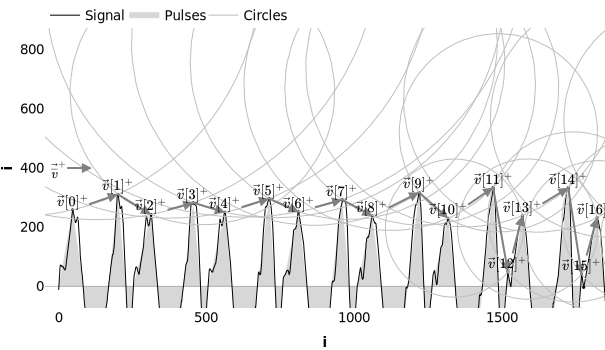
\includegraphics[width=0.8\linewidth]{05Curvatures.pdf}
  \caption{The equivalent circles obtained via the procedure described for the positive frontier. $\theta$, the angle between $ \vec{\overline{v}}^+$ and each of the $\vec{v}_l^+$ is used, as is the horizontal component of each $\vec{v}_l^+$ to obtain the radii of the circles.}
  \label{fig:Curvatures}
\end{figure}

After this procedure one obtains a set of points in $ \mathbb{R}^2 $ where the ordinate represents the instantaneous radius, with its localization in the space of the wave given by the ordinates. Given the robustness of the method, for an average wave of a couple of seconds at an ordinary rate of 44100 $ \mathit{fps} $ the average of the radius values is sufficient to assure the identification of the frontier. However, a curve fitting method can be used in the case of longer waves. An example of the use of the average equivalent circle can be seen in figure \ref{fig:AvgCircle}.

\begin{figure}[ht!]
  \centering
    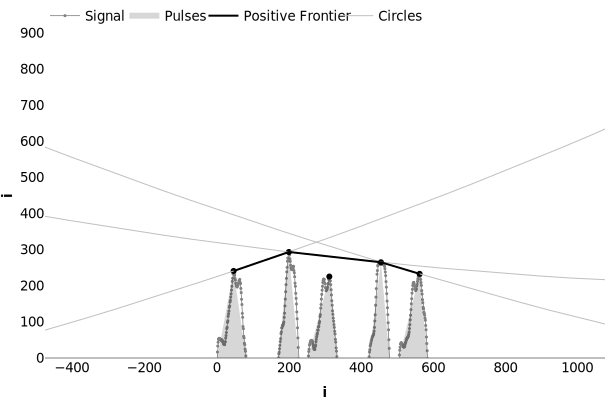
\includegraphics[width=0.8\linewidth]{06AvgCircle.pdf}
  \caption{The positive frontier as obtained by the use of the circle representing the average curvature of the discrete wave illustrated.}
  \label{fig:AvgCircle}
\end{figure}

\section{Results}

Figure \ref{fig:FullFrontiers} illustrates the frontiers obtained to six diverse discrete sound waves, as well as a detail view of a shorter segment for each wave. All waves are records of physical sounds, chosen to represent the applicability of the algorithm in real world scenarios.

We can see that the frontier is satisfactorily detected in harmonic an inharmonic sounds, and presents robustness in relation to the number of samples and the frequencies of the waves.

Besides, the algorithm presents a definition of the position of the cycles of a wave, with which on can, for example, derive its fundamental frequency and phase: using one of the two frontiers, we have $ f = (\#F^\pm - 1) n / (F^\pm[-1] - F^\pm[0])$, where $ \#F^\pm $ denotes the cardinality of the frontier, while $ F^\pm[0] $ and $ F^\pm[-1] $ stand for the frontier's first and last item, respectively.

Similarly, each item of each of the frontiers can be used to estimate the local phase at that location. For the positive frontier, it is necessary to note that, for each item, the following equation holds: $ \cos(\phi + 2 \pi f i / n) = 1 $, and thus $ \phi = k 2 \pi - 2 \pi f i / n $, with $ k \in \mathbb{N } $, while for the negative frontier $ \cos(\phi + 2 \pi f i / n) = -1 $ and $ \phi = k 3 \pi - 2 \pi f i / n) $.

\begin{figure}[ht!]
  \centering
    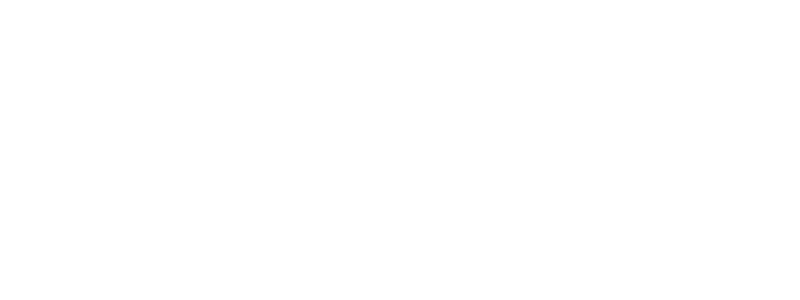
\includegraphics[width=0.8\linewidth]{07FullFrontiers.pdf}
  \caption{Positive and negative frontiers of 6 digital waves, as extracted by the algorithm here presented. For each wave, the region highlighted in black is shown in detail besides the whole wave. For each wave the horizontal axis is the sample number $i$, while the vertical axis is the normalized amplitude. All 6 waves were recorded at 44100 $ \mathit{fps} $.}
  \label{fig:FullFrontiers}
\end{figure}

The impact of the normalization of the wave with the frontiers obtained can be seen in figure \ref{fig:Fourier}, which shows the original and normalized wave in the case of a recording of the key 33 of a piano both in the time and frequency domains.

\begin{figure}[ht!]
  \centering
    \includegraphics[width=0.8\linewidth]{08Fourier.pdf}
  \caption{Original and normalized views of a recording of key 33 (F3, 175 Hz) from a grand piano both in time and frequency domains.}
  \label{fig:Fourier}
\end{figure}

\subsection{Robustness}

Figures \ref{fig:xRobustness} and \ref{fig:yRobustness} illustrate the computational resilience of the algorithm for scaling in both the abscissa and ordinate axes, respectively. This is due to the normalization scheme presented in equation \ref{eq:scale}.

Although important from a theoretical standpoint, this step has a special computational relevance in the case of digital sound waves, as they tend to be composed of a high number of samples in moderate amplitudes, generally normalized between -1 and 1, leading to a numerical disparity between axes.

\begin{figure}[ht!]
  \centering
    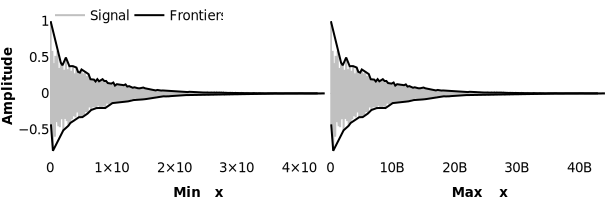
\includegraphics[width=0.8\linewidth]{10xRobustness.pdf}
  \caption{Minimum and maximum scales of the abscissa before computational stability issues arose, for a recording of a drumkit tom.  $ \text{B} = 10^6 $.}
  \label{fig:xRobustness}
\end{figure}

\begin{figure}[ht!]
  \centering
    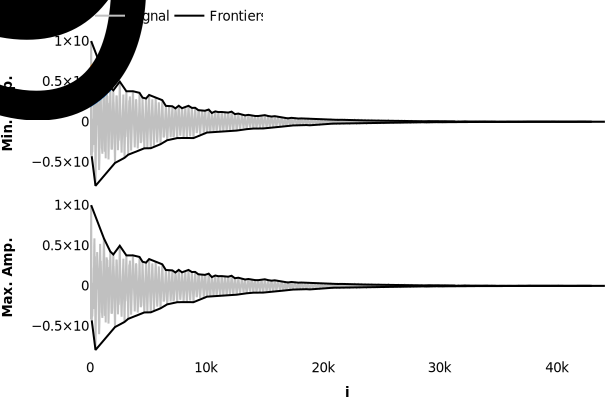
\includegraphics[width=0.8\linewidth]{09yRobustness.pdf}
  \caption{Minimum and maximum values of the amplitude before computational stability issues arose, for a recording of a drumkit tom.}
  \label{fig:yRobustness}
\end{figure}

\subsection{Comparison with traditional algorithms}

Direct comparison with many of the more recent algorithms is made difficult by the unavailability of digital implementations of such works, many designed to process analog signals \parencite[e.g.,][]{2018AssefModeling}.

Nevertheless, insight can be gained from a comparison of the results of the method here proposed with some of the most common envelope extraction algorithms, as cane be seen in figure \ref{fig:Comparison}.

\begin{figure}[ht!]
  \centering
    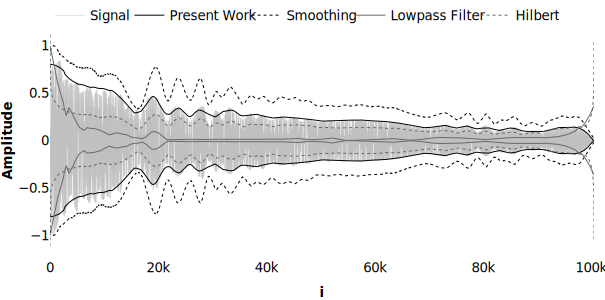
\includegraphics[width=0.8\linewidth]{12Comparison.pdf}
  \caption{Comparison of the algorithm present in this work with the most common methods of digital envelope identification.}
  \label{fig:Comparison}
\end{figure}

For a recording of a guitar bend, we contrast the proposed algorithm with four common approaches of varied complexity: simple smoothing of the rectified original wave, lowpass filtering followed by peak identification and subsequent smoothing, and the extraction of the envelope via Hilbert transform, as presented earlier in the paper, with a previous smoothing of the original wave to avoid the artefacts shown in figure \ref{fig:AnalyticSignal}.

All those methods demanded careful parameter tuning: in the case of filtering, a local cut-off frequency of approximately 88 Hz was used, consisting of one additional parameter to be tuned. For all the other traditional approaches, the Savitzky-Golay smoothing algorithm was used, and the window size was the parameter to be defined.

In the case of the proposed algorithm, the smooth temporal envelope was obtained merging both positive and negative frontiers, that were also smoothed with the same procedure described. Figure \ref{fig:FrontiersToEnvelope} illustrates this process.

\begin{figure}[ht!]
  \centering
    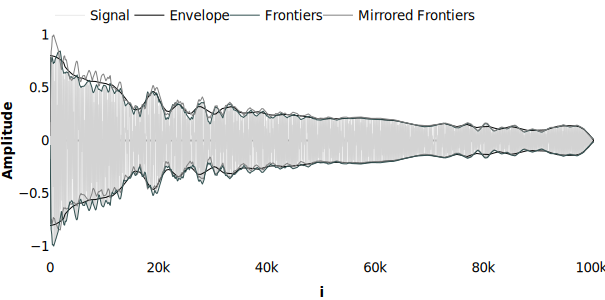
\includegraphics[width=0.8\linewidth]{13FrontiersToEnvelope.pdf}
  \caption{Original positive and negative frontiers in dark gray and their mirrored versions. The temporal envelope, in black, is obtained by merging and approximating both frontiers.}
  \label{fig:FrontiersToEnvelope}
\end{figure}

Table \ref{table:Comparison} presents some computational results. The times are for custom implementations of those methods in the Python programming language. The least mean squares was calculated halving the envelopes presented in figure \ref{fig:Comparison} and comparing then with the rectified absolute wave, so as to avoid the potential influence of an estimated frequency. We can see that, while the algorithm here presented is the most accurate, it's also the most computationally intensive. The connection between alpha-shapes and Delaunay triangulation can be explored in future works as a mean to improve the efficiency of the algorithm.

\begin{table}[ht!]
\centering
\begin{tabular}{ l c c }
\hline
Method & LMS & time(s) \\
\hline
Presented Algorithm & 0.0088 & 4.1507 \\ 
Smoothing           & 0.0123 & 0.1911 \\ 
Lowpass Filter      & 0.0258 & 0.5601 \\ 
Hilbert Transform   & 0.0141 & 0.2599 \\ 
\hline
\end{tabular}
\caption{Comparison of the algorithm present in this work with the most common methods of digital envelope identification.}
\label{table:Comparison}
\end{table}

\section{Discussion}

This work hopes to fill a gap identified by the authors in the context of sound synthesis, where the lack of procedures for the accurate identification of the temporal envelope of arbitrary waves consists of an obstacle to the complete description, and eventual manipulation of signals.

While relevant in its own accord, the procedure here presented isolates the individual cycles of a wave, pinpointing them in the time domain. Due to that, a rich set of theoretical advancements, of whose an example was given in the preceding section, can be built upon this initial building block.

With the knowledge of the exact position and characteristics of the cycles of a wave, one can investigate its evolution in time, in terms of frequency content for example, free from the potencial interference of a modulating wave; in other words, one can have a very satisfactory view of the instantaneous frequencies and phase of an arbitrary wave and its evolution in time, providing a way to bridge the gap between time domain and frequency domain interpretations.

\section{References}

\printbibliography[heading=none]

\end{document}
